% Autômato finito determinístico
% Feito para o ÉguaTeX (eguatex.com.br). Uso livre (CC0 1.0).
%
% Compile e pronto: sai só a figura, em PDF.
% Para pôr no seu trabalho, use o PDF com \includegraphics ou copie
% o bloco tikzpicture para dentro de uma figure e ponha no preâmbulo
% \usepackage{tikz} e \usetikzlibrary{automata, positioning}.
%
% Exemplo: aceita as cadeias de 0 e 1 que terminam em 01.
\documentclass[tikz,border=4pt]{standalone}
\usepackage[T1]{fontenc}
\usepackage{lmodern}
\usetikzlibrary{automata, positioning}

\begin{document}
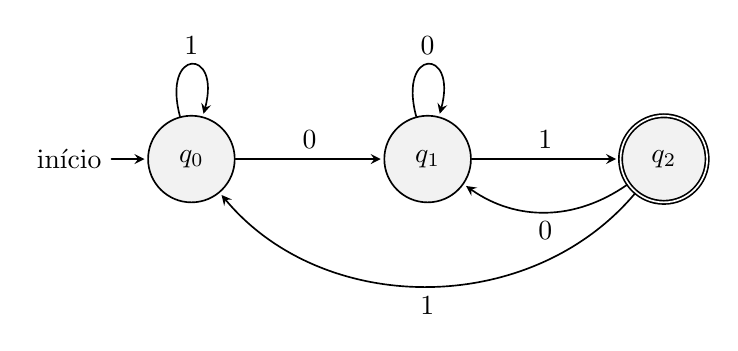
\begin{tikzpicture}[>=stealth, line cap=round, shorten >=1pt, auto,
  node distance=3cm, on grid, semithick,
  every state/.style={fill=black!5, minimum size=1.1cm},
  initial text={início}]

% Estados: "initial" marca o inicial e "accepting" os de aceitação.
\node[state, initial]   (q0)                {$q_0$};
\node[state]            (q1) [right=of q0]  {$q_1$};
\node[state, accepting] (q2) [right=of q1]  {$q_2$};

% Transições: de, para e o símbolo lido.
\path[->]
  (q0) edge [loop above]       node {$1$} ()
       edge                    node {$0$} (q1)
  (q1) edge [loop above]       node {$0$} ()
       edge                    node {$1$} (q2)
  (q2) edge [bend left=35]     node {$0$} (q1)
       edge [bend left=50]     node {$1$} (q0);
\end{tikzpicture}
\end{document}
